\documentclass[conference]{IEEEtran}
\IEEEoverridecommandlockouts
% The preceding line is only needed to identify funding in the first footnote. If that is unneeded, please comment it out.
\usepackage{cite}
\usepackage[ngerman]{babel}
\usepackage[utf8]{inputenc}
\usepackage{amsmath,amssymb,amsfonts}
\usepackage{algorithmic}
\usepackage{graphicx}
\usepackage{textcomp}
\usepackage{xcolor}
\usepackage{listings}


\definecolor{pblue}{rgb}{0.13,0.13,1}
\definecolor{pgreen}{rgb}{0,0.5,0}
\definecolor{pred}{rgb}{0.9,0,0}
\definecolor{pgrey}{rgb}{0.46,0.45,0.48}
\lstset{language=Java,
	showspaces=false,
	showtabs=false,
	breaklines=true,
	tabsize=2,
	showstringspaces=false,
	breakatwhitespace=true,
	commentstyle=\color{pgreen},
	keywordstyle=\color{pblue},
	stringstyle=\color{pred},
	basicstyle=\ttfamily
}


\usepackage{url}
\def\BibTeX{{\rm B\kern-.05em{\sc i\kern-.025em b}\kern-.08em
		T\kern-.1667em\lower.7ex\hbox{E}\kern-.125emX}}
\begin{document}
	
	\title{Computational Geometry - Abgabe 4}
	
	\author{\IEEEauthorblockN{1\textsuperscript{st} Bartolovic Eduard}
		\IEEEauthorblockA{\textit{Hochschule München} \\
			München, Deutschland \\
			eduard.bartolovic0@hm.edu}
	}
	
	\maketitle
	
	\begin{abstract}
		
		
	\end{abstract}
	
	\section{Konvexe Hülle}
	 N*logN Quickhull mit Worstcase $n^2$
	
	Höher: 
	
	Eine symmetrische Anordnung der Punkte besitzt jedoch eine höhere Wahrscheinlichkeit die Best Case (bester Fall) Laufzeitschranke von $\mathcal{O}(n * \log(n))$ zu verlassen und deutlich langsamer zu sein. 
	%Quickhull is a method of computing the convex hull of a finite set of points in n-dimensional %space. It uses a divide and conquer approach similar to that of quicksort, from which its name %derives. Its worst case complexity for 2-dimensional and 3-dimensional space is considered to be %O ( n log ⁡ ( r ) ) {\displaystyle O(n\log(r))} {\displaystyle O(n\log(r))}, where n %{\displaystyle n} n is the number of input points and r {\displaystyle r} r is the number of %processed points.[1] However, unlike quicksort, there is no obvious way to convert quickhull %into a randomized algorithm. Nevertheless, there exist works from Smoothed Analysis which tell %us that the 2-dimensional Quick hull algorithm has expected runtime O ( n log ⁡ ( n ) ) %{\displaystyle O(n\log(n))} O(n\log(n))
	
	\begin{figure}[h]
		\begin{center}
			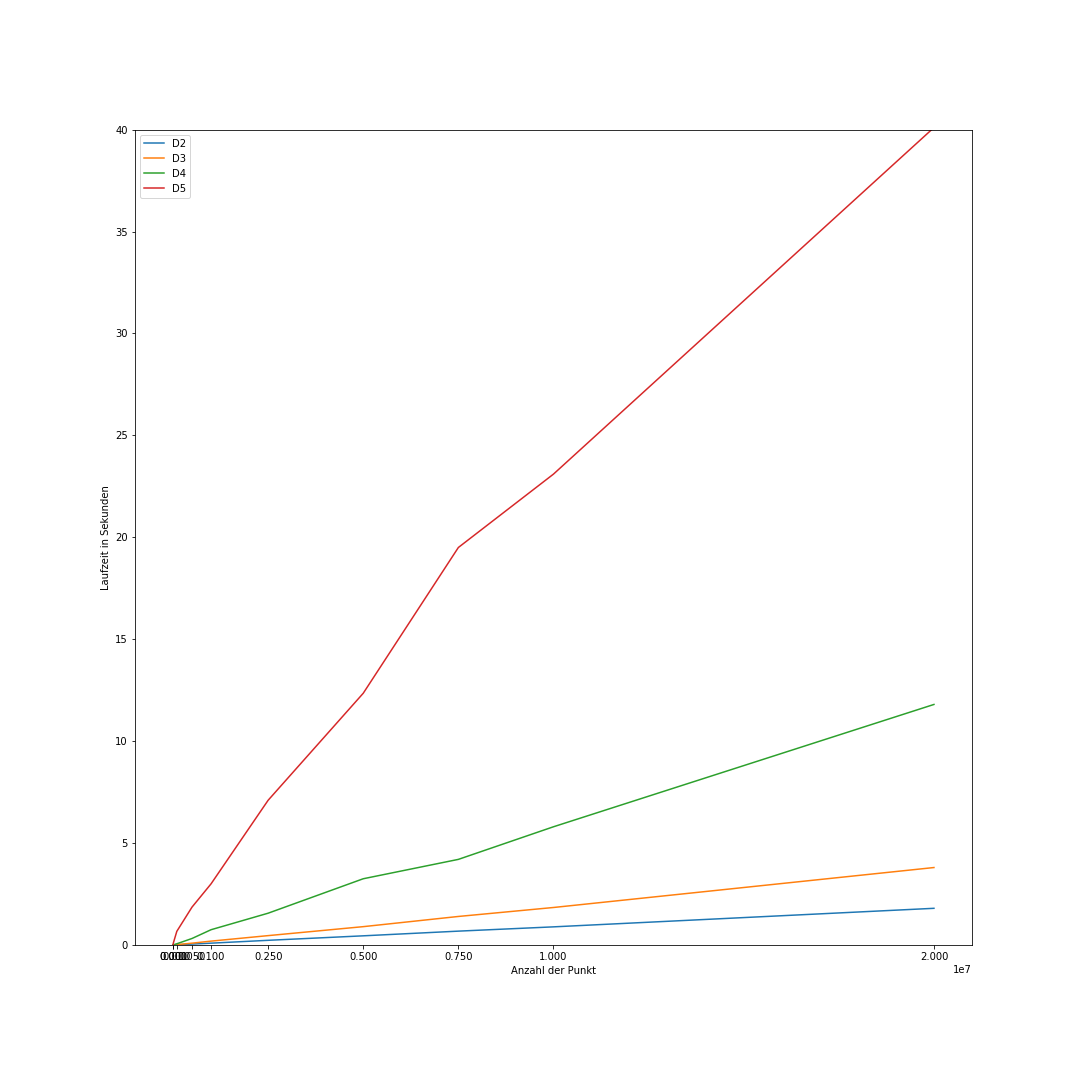
\includegraphics[width=6cm]{index.png}
			\caption{Normal}
			\label{figure_1}
		\end{center}
	\end{figure}
	\begin{figure}[h]
		\begin{center}
			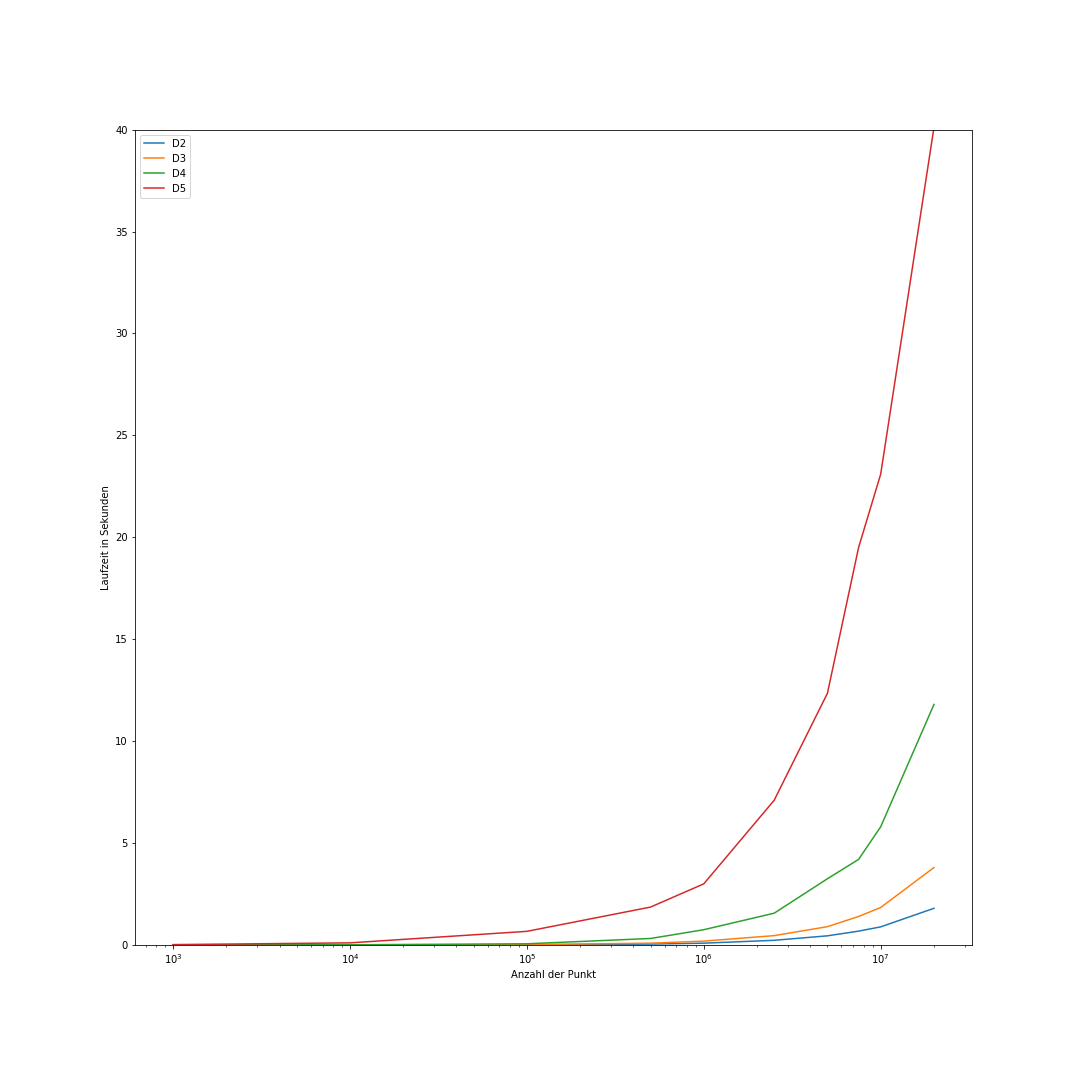
\includegraphics[width=6cm]{index2.png}
			\caption{X As log scale}
			\label{figure_2}
		\end{center}
	\end{figure}
	
	
	\begin{thebibliography}{00}
		\bibitem{b2}https://docs.oracle.com/javase/8/docs/api/java/util/PriorityQueue.html
		\bibitem{b1}https://docs.oracle.com/javase/7/docs/api/java/util/TreeMap.html
	\end{thebibliography}
	
	
	
	\section{Anhang}

	Berechnung der Fläche eines Bundeslandes:
	\begin{lstlisting}[basicstyle=\tiny]
	public double calculateArea(){
		double sum = 0;
		for(Polygon p : areas){
			boolean isInside = false;
			for(Polygon p2 : areas){
				//Check if Hole
				if(!p.equals(p2) && p.isPolygonInside(p2) ){ 
					isInside = true;
					break;
				}   
			}
			if(isInside)
				sum -= Math.abs(p.calculateArea());
			else
				sum += Math.abs(p.calculateArea());
		}
		return sum;
	}
	\end{lstlisting}	

\end{document}
